\documentclass[1p]{elsarticle_modified}
%\bibliographystyle{elsarticle-num}

%\usepackage[colorlinks]{hyperref}
%\usepackage{abbrmath_seonhwa} %\Abb, \Ascr, \Acal ,\Abf, \Afrak
\usepackage{amsfonts}
\usepackage{amssymb}
\usepackage{amsmath}
\usepackage{amsthm}
\usepackage{scalefnt}
\usepackage{amsbsy}
\usepackage{kotex}
\usepackage{caption}
\usepackage{subfig}
\usepackage{color}
\usepackage{graphicx}
\usepackage{xcolor} %% white, black, red, green, blue, cyan, magenta, yellow
\usepackage{float}
\usepackage{setspace}
\usepackage{hyperref}

\usepackage{tikz}
\usetikzlibrary{arrows}

\usepackage{multirow}
\usepackage{array} % fixed length table
\usepackage{hhline}

%%%%%%%%%%%%%%%%%%%%%
\makeatletter
\renewcommand*\env@matrix[1][\arraystretch]{%
	\edef\arraystretch{#1}%
	\hskip -\arraycolsep
	\let\@ifnextchar\new@ifnextchar
	\array{*\c@MaxMatrixCols c}}
\makeatother %https://tex.stackexchange.com/questions/14071/how-can-i-increase-the-line-spacing-in-a-matrix
%%%%%%%%%%%%%%%

\usepackage[normalem]{ulem}

\newcommand{\msout}[1]{\ifmmode\text{\sout{\ensuremath{#1}}}\else\sout{#1}\fi}
%SOURCE: \msout is \stkout macro in https://tex.stackexchange.com/questions/20609/strikeout-in-math-mode

\newcommand{\cancel}[1]{
	\ifmmode
	{\color{red}\msout{#1}}
	\else
	{\color{red}\sout{#1}}
	\fi
}

\newcommand{\add}[1]{
	{\color{blue}\uwave{#1}}
}

\newcommand{\replace}[2]{
	\ifmmode
	{\color{red}\msout{#1}}{\color{blue}\uwave{#2}}
	\else
	{\color{red}\sout{#1}}{\color{blue}\uwave{#2}}
	\fi
}

\newcommand{\Sol}{\mathcal{S}} %segment
\newcommand{\D}{D} %diagram
\newcommand{\A}{\mathcal{A}} %arc


%%%%%%%%%%%%%%%%%%%%%%%%%%%%%5 test

\def\sl{\operatorname{\textup{SL}}(2,\Cbb)}
\def\psl{\operatorname{\textup{PSL}}(2,\Cbb)}
\def\quan{\mkern 1mu \triangleright \mkern 1mu}

\theoremstyle{definition}
\newtheorem{thm}{Theorem}[section]
\newtheorem{prop}[thm]{Proposition}
\newtheorem{lem}[thm]{Lemma}
\newtheorem{ques}[thm]{Question}
\newtheorem{cor}[thm]{Corollary}
\newtheorem{defn}[thm]{Definition}
\newtheorem{exam}[thm]{Example}
\newtheorem{rmk}[thm]{Remark}
\newtheorem{alg}[thm]{Algorithm}

\newcommand{\I}{\sqrt{-1}}
\begin{document}

%\begin{frontmatter}
%
%\title{Boundary parabolic representations of knots up to 8 crossings}
%
%%% Group authors per affiliation:
%\author{Yunhi Cho} 
%\address{Department of Mathematics, University of Seoul, Seoul, Korea}
%\ead{yhcho@uos.ac.kr}
%
%
%\author{Seonhwa Kim} %\fnref{s_kim}}
%\address{Center for Geometry and Physics, Institute for Basic Science, Pohang, 37673, Korea}
%\ead{ryeona17@ibs.re.kr}
%
%\author{Hyuk Kim}
%\address{Department of Mathematical Sciences, Seoul National University, Seoul 08826, Korea}
%\ead{hyukkim@snu.ac.kr}
%
%\author{Seokbeom Yoon}
%\address{Department of Mathematical Sciences, Seoul National University, Seoul, 08826,  Korea}
%\ead{sbyoon15@snu.ac.kr}
%
%\begin{abstract}
%We find all boundary parabolic representation of knots up to 8 crossings.
%
%\end{abstract}
%\begin{keyword}
%    \MSC[2010] 57M25 
%\end{keyword}
%
%\end{frontmatter}

%\linenumbers
%\tableofcontents
%
\newcommand\colored[1]{\textcolor{white}{\rule[-0.35ex]{0.8em}{1.4ex}}\kern-0.8em\color{red} #1}%
%\newcommand\colored[1]{\textcolor{white}{ #1}\kern-2.17ex	\textcolor{white}{ #1}\kern-1.81ex	\textcolor{white}{ #1}\kern-2.15ex\color{red}#1	}

{\Large $\underline{12a_{0739}~(K12a_{0739})}$}

\setlength{\tabcolsep}{10pt}
\renewcommand{\arraystretch}{1.6}
\vspace{1cm}\begin{tabular}{m{100pt}>{\centering\arraybackslash}m{274pt}}
\multirow{5}{120pt}{
	\centering
	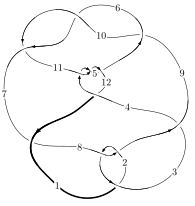
\includegraphics[width=112pt]{../../../GIT/diagram.site/Diagrams/png/1540_12a_0739.png}\\
\ \ \ A knot diagram\footnotemark}&
\allowdisplaybreaks
\textbf{Linearized knot diagam} \\
\cline{2-2}
 &
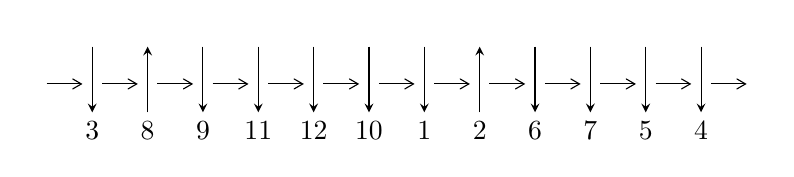
\begin{tikzpicture}[x=20pt, y=17pt]
	% nodes
	\node (C0) at (0, 0) {};
	\node (C1) at (1, 0) {};
	\node (C1U) at (1, +1) {};
	\node (C1D) at (1, -1) {3};

	\node (C2) at (2, 0) {};
	\node (C2U) at (2, +1) {};
	\node (C2D) at (2, -1) {8};

	\node (C3) at (3, 0) {};
	\node (C3U) at (3, +1) {};
	\node (C3D) at (3, -1) {9};

	\node (C4) at (4, 0) {};
	\node (C4U) at (4, +1) {};
	\node (C4D) at (4, -1) {11};

	\node (C5) at (5, 0) {};
	\node (C5U) at (5, +1) {};
	\node (C5D) at (5, -1) {12};

	\node (C6) at (6, 0) {};
	\node (C6U) at (6, +1) {};
	\node (C6D) at (6, -1) {10};

	\node (C7) at (7, 0) {};
	\node (C7U) at (7, +1) {};
	\node (C7D) at (7, -1) {1};

	\node (C8) at (8, 0) {};
	\node (C8U) at (8, +1) {};
	\node (C8D) at (8, -1) {2};

	\node (C9) at (9, 0) {};
	\node (C9U) at (9, +1) {};
	\node (C9D) at (9, -1) {6};

	\node (C10) at (10, 0) {};
	\node (C10U) at (10, +1) {};
	\node (C10D) at (10, -1) {7};

	\node (C11) at (11, 0) {};
	\node (C11U) at (11, +1) {};
	\node (C11D) at (11, -1) {5};

	\node (C12) at (12, 0) {};
	\node (C12U) at (12, +1) {};
	\node (C12D) at (12, -1) {4};
	\node (C13) at (13, 0) {};

	% arrows
	\draw[->,>={angle 60}]
	(C0) edge (C1) (C1) edge (C2) (C2) edge (C3) (C3) edge (C4) (C4) edge (C5) (C5) edge (C6) (C6) edge (C7) (C7) edge (C8) (C8) edge (C9) (C9) edge (C10) (C10) edge (C11) (C11) edge (C12) (C12) edge (C13) ;	\draw[->,>=stealth]
	(C1U) edge (C1D) (C2D) edge (C2U) (C3U) edge (C3D) (C4U) edge (C4D) (C5U) edge (C5D) (C6U) edge (C6D) (C7U) edge (C7D) (C8D) edge (C8U) (C9U) edge (C9D) (C10U) edge (C10D) (C11U) edge (C11D) (C12U) edge (C12D) ;
	\end{tikzpicture} \\
\hhline{~~} \\& 
\textbf{Solving Sequence} \\ \cline{2-2} 
 &
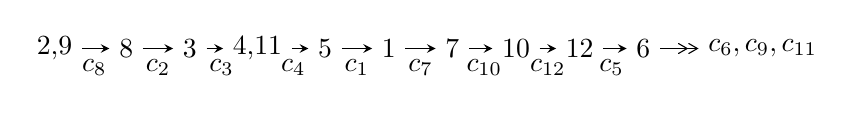
\begin{tikzpicture}[x=23pt, y=7pt]
	% node
	\node (A0) at (-1/8, 0) {2,9};
	\node (A1) at (1, 0) {8};
	\node (A2) at (2, 0) {3};
	\node (A3) at (49/16, 0) {4,11};
	\node (A4) at (33/8, 0) {5};
	\node (A5) at (41/8, 0) {1};
	\node (A6) at (49/8, 0) {7};
	\node (A7) at (57/8, 0) {10};
	\node (A8) at (65/8, 0) {12};
	\node (A9) at (73/8, 0) {6};
	\node (C1) at (1/2, -1) {$c_{8}$};
	\node (C2) at (3/2, -1) {$c_{2}$};
	\node (C3) at (5/2, -1) {$c_{3}$};
	\node (C4) at (29/8, -1) {$c_{4}$};
	\node (C5) at (37/8, -1) {$c_{1}$};
	\node (C6) at (45/8, -1) {$c_{7}$};
	\node (C7) at (53/8, -1) {$c_{10}$};
	\node (C8) at (61/8, -1) {$c_{12}$};
	\node (C9) at (69/8, -1) {$c_{5}$};
	\node (A10) at (11, 0) {$c_{6},c_{9},c_{11}$};

	% edge
	\draw[->,>=stealth]	
	(A0) edge (A1) (A1) edge (A2) (A2) edge (A3) (A3) edge (A4) (A4) edge (A5) (A5) edge (A6) (A6) edge (A7) (A7) edge (A8) (A8) edge (A9) ;
	\draw[->>,>={angle 60}]	
	(A9) edge (A10);
\end{tikzpicture} \\ 

\end{tabular} \\

\footnotetext{
The image of knot diagram is generated by the software ``\textbf{Draw programme}" developed by Andrew Bartholomew(\url{http://www.layer8.co.uk/maths/draw/index.htm\#Running-draw}), where we modified some parts for our purpose(\url{https://github.com/CATsTAILs/LinksPainter}).
}\phantom \\ \newline 
\centering \textbf{Ideals for irreducible components\footnotemark of $X_{\text{par}}$} 
 
\begin{align*}
I^u_{1}&=\langle 
3 u^{31}+6 u^{30}+\cdots+b+3,\;-7 u^{31}-17 u^{30}+\cdots+2 a-6,\;u^{32}+3 u^{31}+\cdots+6 u+2\rangle \\
I^u_{2}&=\langle 
u^{23} a+7 u^{23}+\cdots- a-50,\;2 u^{23} a- u^{23}+\cdots+a^2- a,\;u^{24}- u^{23}+\cdots-2 u+1\rangle \\
I^u_{3}&=\langle 
b-1,\;u^3+2 u^2+2 a+4,\;u^4+2 u^2+2\rangle \\
\\
I^v_{1}&=\langle 
a,\;b-1,\;v+1\rangle \\
\end{align*}
\raggedright * 4 irreducible components of $\dim_{\mathbb{C}}=0$, with total 85 representations.\\
\footnotetext{All coefficients of polynomials are rational numbers. But the coefficients are sometimes approximated in decimal forms when there is not enough margin.}
\newpage
\renewcommand{\arraystretch}{1}
\centering \section*{I. $I^u_{1}= \langle 3 u^{31}+6 u^{30}+\cdots+b+3,\;-7 u^{31}-17 u^{30}+\cdots+2 a-6,\;u^{32}+3 u^{31}+\cdots+6 u+2 \rangle$}
\flushleft \textbf{(i) Arc colorings}\\
\begin{tabular}{m{7pt} m{180pt} m{7pt} m{180pt} }
\flushright $a_{2}=$&$\begin{pmatrix}0\\u\end{pmatrix}$ \\
\flushright $a_{9}=$&$\begin{pmatrix}1\\0\end{pmatrix}$ \\
\flushright $a_{8}=$&$\begin{pmatrix}1\\u^2\end{pmatrix}$ \\
\flushright $a_{3}=$&$\begin{pmatrix}u\\u^3+u\end{pmatrix}$ \\
\flushright $a_{4}=$&$\begin{pmatrix}- u^3\\u^3+u\end{pmatrix}$ \\
\flushright $a_{11}=$&$\begin{pmatrix}\frac{7}{2} u^{31}+\frac{17}{2} u^{30}+\cdots+10 u+3\\-3 u^{31}-6 u^{30}+\cdots-6 u-3\end{pmatrix}$ \\
\flushright $a_{5}=$&$\begin{pmatrix}-\frac{1}{2} u^{31}-\frac{3}{2} u^{30}+\cdots-2 u-1\\- u^{29}- u^{28}+\cdots- u-1\end{pmatrix}$ \\
\flushright $a_{1}=$&$\begin{pmatrix}u^3\\u^5+u^3+u\end{pmatrix}$ \\
\flushright $a_{7}=$&$\begin{pmatrix}- u^6- u^4+1\\- u^8-2 u^6-2 u^4\end{pmatrix}$ \\
\flushright $a_{10}=$&$\begin{pmatrix}\frac{3}{2} u^{31}+\frac{7}{2} u^{30}+\cdots+4 u+2\\- u^{31}-2 u^{30}+\cdots-2 u-1\end{pmatrix}$ \\
\flushright $a_{12}=$&$\begin{pmatrix}u^{11}+2 u^9+2 u^7+u^3\\- u^{11}-3 u^9-4 u^7- u^5+u^3+u\end{pmatrix}$ \\
\flushright $a_{6}=$&$\begin{pmatrix}-\frac{1}{2} u^{31}-\frac{3}{2} u^{30}+\cdots-4 u-3\\- u^{29}- u^{28}+\cdots-2 u-1\end{pmatrix}$\\&\end{tabular}
\flushleft \textbf{(ii) Obstruction class $= -1$}\\~\\
\flushleft \textbf{(iii) Cusp Shapes $= 2 u^{30}+6 u^{29}+24 u^{28}+48 u^{27}+118 u^{26}+184 u^{25}+346 u^{24}+442 u^{23}+680 u^{22}+734 u^{21}+948 u^{20}+882 u^{19}+940 u^{18}+750 u^{17}+614 u^{16}+384 u^{15}+160 u^{14}-26 u^{13}-174 u^{12}-266 u^{11}-274 u^{10}-286 u^9-220 u^8-170 u^7-92 u^6-46 u^5-16 u^4-6 u^3+12 u^2+14 u$}\\~\\
\newpage\renewcommand{\arraystretch}{1}
\flushleft \textbf{(iv) u-Polynomials at the component}\newline \\
\begin{tabular}{m{50pt}|m{274pt}}
Crossings & \hspace{64pt}u-Polynomials at each crossing \\
\hline $$\begin{aligned}c_{1}\end{aligned}$$&$\begin{aligned}
&u^{32}+17 u^{31}+\cdots+4 u+4
\end{aligned}$\\
\hline $$\begin{aligned}c_{2},c_{8}\end{aligned}$$&$\begin{aligned}
&u^{32}-3 u^{31}+\cdots-6 u+2
\end{aligned}$\\
\hline $$\begin{aligned}c_{3},c_{7}\end{aligned}$$&$\begin{aligned}
&u^{32}+3 u^{31}+\cdots+186 u+34
\end{aligned}$\\
\hline $$\begin{aligned}c_{4},c_{5},c_{6}\\c_{9},c_{10},c_{11}\end{aligned}$$&$\begin{aligned}
&u^{32}+u^{31}+\cdots-2 u-1
\end{aligned}$\\
\hline $$\begin{aligned}c_{12}\end{aligned}$$&$\begin{aligned}
&u^{32}-3 u^{31}+\cdots+256 u+256
\end{aligned}$\\
\hline
\end{tabular}\\~\\
\newpage\renewcommand{\arraystretch}{1}
\flushleft \textbf{(v) Riley Polynomials at the component}\newline \\
\begin{tabular}{m{50pt}|m{274pt}}
Crossings & \hspace{64pt}Riley Polynomials at each crossing \\
\hline $$\begin{aligned}c_{1}\end{aligned}$$&$\begin{aligned}
&y^{32}-3 y^{31}+\cdots-240 y+16
\end{aligned}$\\
\hline $$\begin{aligned}c_{2},c_{8}\end{aligned}$$&$\begin{aligned}
&y^{32}+17 y^{31}+\cdots+4 y+4
\end{aligned}$\\
\hline $$\begin{aligned}c_{3},c_{7}\end{aligned}$$&$\begin{aligned}
&y^{32}-23 y^{31}+\cdots+1988 y+1156
\end{aligned}$\\
\hline $$\begin{aligned}c_{4},c_{5},c_{6}\\c_{9},c_{10},c_{11}\end{aligned}$$&$\begin{aligned}
&y^{32}-35 y^{31}+\cdots-8 y+1
\end{aligned}$\\
\hline $$\begin{aligned}c_{12}\end{aligned}$$&$\begin{aligned}
&y^{32}+y^{31}+\cdots-1441792 y+65536
\end{aligned}$\\
\hline
\end{tabular}\\~\\
\newpage\flushleft \textbf{(vi) Complex Volumes and Cusp Shapes}
$$\begin{array}{c|c|c}  
\text{Solutions to }I^u_{1}& \I (\text{vol} + \sqrt{-1}CS) & \text{Cusp shape}\\
 \hline 
\begin{aligned}
u &= \phantom{-}0.530176 + 0.767965 I \\
a &= -0.333698 + 1.088190 I \\
b &= -1.227720 - 0.174945 I\end{aligned}
 & \phantom{-}3.24325 + 2.15228 I & -1.95940 - 4.22418 I \\ \hline\begin{aligned}
u &= \phantom{-}0.530176 - 0.767965 I \\
a &= -0.333698 - 1.088190 I \\
b &= -1.227720 + 0.174945 I\end{aligned}
 & \phantom{-}3.24325 - 2.15228 I & -1.95940 + 4.22418 I \\ \hline\begin{aligned}
u &= \phantom{-}0.600367 + 0.882410 I \\
a &= \phantom{-}1.053060 - 0.667414 I \\
b &= \phantom{-}0.99155 + 1.32550 I\end{aligned}
 & -5.84755 + 9.45240 I & -12.6198 - 8.2074 I \\ \hline\begin{aligned}
u &= \phantom{-}0.600367 - 0.882410 I \\
a &= \phantom{-}1.053060 + 0.667414 I \\
b &= \phantom{-}0.99155 - 1.32550 I\end{aligned}
 & -5.84755 - 9.45240 I & -12.6198 + 8.2074 I \\ \hline\begin{aligned}
u &= \phantom{-}0.646120 + 0.645507 I \\
a &= -0.580073 - 1.083300 I \\
b &= \phantom{-}0.852194 - 1.117410 I\end{aligned}
 & -5.16481 - 4.62443 I & -11.58848 + 2.31548 I \\ \hline\begin{aligned}
u &= \phantom{-}0.646120 - 0.645507 I \\
a &= -0.580073 + 1.083300 I \\
b &= \phantom{-}0.852194 + 1.117410 I\end{aligned}
 & -5.16481 + 4.62443 I & -11.58848 - 2.31548 I \\ \hline\begin{aligned}
u &= -0.131686 + 1.135040 I \\
a &= -0.83751 + 1.33294 I \\
b &= \phantom{-}0.240682 - 1.143010 I\end{aligned}
 & -11.15830 - 4.71723 I & -19.1935 + 3.5978 I \\ \hline\begin{aligned}
u &= -0.131686 - 1.135040 I \\
a &= -0.83751 - 1.33294 I \\
b &= \phantom{-}0.240682 + 1.143010 I\end{aligned}
 & -11.15830 + 4.71723 I & -19.1935 - 3.5978 I \\ \hline\begin{aligned}
u &= -0.837356 + 0.165249 I \\
a &= \phantom{-}0.404130 - 0.561898 I \\
b &= \phantom{-}1.02549 + 1.88978 I\end{aligned}
 & -9.6605 + 10.4842 I & -13.3472 - 5.6777 I \\ \hline\begin{aligned}
u &= -0.837356 - 0.165249 I \\
a &= \phantom{-}0.404130 + 0.561898 I \\
b &= \phantom{-}1.02549 - 1.88978 I\end{aligned}
 & -9.6605 - 10.4842 I & -13.3472 + 5.6777 I\\
 \hline 
 \end{array}$$\newpage$$\begin{array}{c|c|c}  
\text{Solutions to }I^u_{1}& \I (\text{vol} + \sqrt{-1}CS) & \text{Cusp shape}\\
 \hline 
\begin{aligned}
u &= \phantom{-}0.850182\phantom{ +0.000000I} \\
a &= -0.699857\phantom{ +0.000000I} \\
b &= -0.827456\phantom{ +0.000000I}\end{aligned}
 & -14.5114\phantom{ +0.000000I} & -16.1110\phantom{ +0.000000I} \\ \hline\begin{aligned}
u &= -0.716975 + 0.384483 I \\
a &= -0.620707 - 0.541693 I \\
b &= \phantom{-}0.537816 - 0.772266 I\end{aligned}
 & -6.35392 - 2.54841 I & -12.91352 + 2.61370 I \\ \hline\begin{aligned}
u &= -0.716975 - 0.384483 I \\
a &= -0.620707 + 0.541693 I \\
b &= \phantom{-}0.537816 + 0.772266 I\end{aligned}
 & -6.35392 + 2.54841 I & -12.91352 - 2.61370 I \\ \hline\begin{aligned}
u &= -0.556688 + 1.075410 I \\
a &= -1.58889 + 0.49107 I \\
b &= \phantom{-}0.474528 + 0.553995 I\end{aligned}
 & -8.36419 - 2.29995 I & -16.4016 + 1.9872 I \\ \hline\begin{aligned}
u &= -0.556688 - 1.075410 I \\
a &= -1.58889 - 0.49107 I \\
b &= \phantom{-}0.474528 - 0.553995 I\end{aligned}
 & -8.36419 + 2.29995 I & -16.4016 - 1.9872 I \\ \hline\begin{aligned}
u &= \phantom{-}0.446730 + 1.133610 I \\
a &= -0.174401 - 0.268039 I \\
b &= \phantom{-}0.451030 - 0.097453 I\end{aligned}
 & -4.05143 + 3.92335 I & -11.83314 - 4.97716 I \\ \hline\begin{aligned}
u &= \phantom{-}0.446730 - 1.133610 I \\
a &= -0.174401 + 0.268039 I \\
b &= \phantom{-}0.451030 + 0.097453 I\end{aligned}
 & -4.05143 - 3.92335 I & -11.83314 + 4.97716 I \\ \hline\begin{aligned}
u &= -0.385111 + 1.156080 I \\
a &= \phantom{-}1.50345 + 1.00275 I \\
b &= -0.605346 - 0.873356 I\end{aligned}
 & -2.81095 - 0.89291 I & -9.61808 - 1.56697 I \\ \hline\begin{aligned}
u &= -0.385111 - 1.156080 I \\
a &= \phantom{-}1.50345 - 1.00275 I \\
b &= -0.605346 + 0.873356 I\end{aligned}
 & -2.81095 + 0.89291 I & -9.61808 + 1.56697 I \\ \hline\begin{aligned}
u &= -0.727485 + 0.163192 I \\
a &= \phantom{-}0.025322 + 0.657062 I \\
b &= -0.937084 - 0.752441 I\end{aligned}
 & \phantom{-}0.91865 + 2.74283 I & -4.47712 - 4.42713 I\\
 \hline 
 \end{array}$$\newpage$$\begin{array}{c|c|c}  
\text{Solutions to }I^u_{1}& \I (\text{vol} + \sqrt{-1}CS) & \text{Cusp shape}\\
 \hline 
\begin{aligned}
u &= -0.727485 - 0.163192 I \\
a &= \phantom{-}0.025322 - 0.657062 I \\
b &= -0.937084 + 0.752441 I\end{aligned}
 & \phantom{-}0.91865 - 2.74283 I & -4.47712 + 4.42713 I \\ \hline\begin{aligned}
u &= -0.156809 + 0.717859 I \\
a &= \phantom{-}0.551971 - 0.300182 I \\
b &= \phantom{-}0.009711 + 0.252381 I\end{aligned}
 & -0.500387 - 0.882970 I & -9.10822 + 7.52488 I \\ \hline\begin{aligned}
u &= -0.156809 - 0.717859 I \\
a &= \phantom{-}0.551971 + 0.300182 I \\
b &= \phantom{-}0.009711 - 0.252381 I\end{aligned}
 & -0.500387 + 0.882970 I & -9.10822 - 7.52488 I \\ \hline\begin{aligned}
u &= -0.502524 + 1.164790 I \\
a &= -0.02663 - 2.31078 I \\
b &= -1.016320 + 0.969217 I\end{aligned}
 & -1.97783 - 7.36348 I & -8.22078 + 7.59115 I \\ \hline\begin{aligned}
u &= -0.502524 - 1.164790 I \\
a &= -0.02663 + 2.31078 I \\
b &= -1.016320 - 0.969217 I\end{aligned}
 & -1.97783 + 7.36348 I & -8.22078 - 7.59115 I \\ \hline\begin{aligned}
u &= -0.355660 + 1.231240 I \\
a &= -1.84106 - 2.12601 I \\
b &= \phantom{-}0.82482 + 1.97592 I\end{aligned}
 & -13.9647 + 6.4949 I & -17.9768 - 2.7490 I \\ \hline\begin{aligned}
u &= -0.355660 - 1.231240 I \\
a &= -1.84106 + 2.12601 I \\
b &= \phantom{-}0.82482 - 1.97592 I\end{aligned}
 & -13.9647 - 6.4949 I & -17.9768 + 2.7490 I \\ \hline\begin{aligned}
u &= -0.529210 + 1.200000 I \\
a &= \phantom{-}1.21068 + 3.02446 I \\
b &= \phantom{-}1.12053 - 2.00398 I\end{aligned}
 & -12.7401 - 15.4900 I & -16.2477 + 8.8219 I \\ \hline\begin{aligned}
u &= -0.529210 - 1.200000 I \\
a &= \phantom{-}1.21068 - 3.02446 I \\
b &= \phantom{-}1.12053 + 2.00398 I\end{aligned}
 & -12.7401 + 15.4900 I & -16.2477 - 8.8219 I \\ \hline\begin{aligned}
u &= \phantom{-}0.455444 + 1.234730 I \\
a &= \phantom{-}0.384015 + 0.486298 I \\
b &= -0.986970 + 0.213554 I\end{aligned}
 & -18.2324 + 4.6426 I & -19.4334 - 3.2455 I\\
 \hline 
 \end{array}$$\newpage$$\begin{array}{c|c|c}  
\text{Solutions to }I^u_{1}& \I (\text{vol} + \sqrt{-1}CS) & \text{Cusp shape}\\
 \hline 
\begin{aligned}
u &= \phantom{-}0.455444 - 1.234730 I \\
a &= \phantom{-}0.384015 - 0.486298 I \\
b &= -0.986970 - 0.213554 I\end{aligned}
 & -18.2324 - 4.6426 I & -19.4334 + 3.2455 I \\ \hline\begin{aligned}
u &= \phantom{-}0.591155\phantom{ +0.000000I} \\
a &= \phantom{-}0.440555\phantom{ +0.000000I} \\
b &= \phantom{-}0.317636\phantom{ +0.000000I}\end{aligned}
 & -1.06479\phantom{ +0.000000I} & -10.0120\phantom{ +0.000000I}\\
 \hline 
 \end{array}$$\newpage\newpage\renewcommand{\arraystretch}{1}
\centering \section*{II. $I^u_{2}= \langle u^{23} a+7 u^{23}+\cdots- a-50,\;2 u^{23} a- u^{23}+\cdots+a^2- a,\;u^{24}- u^{23}+\cdots-2 u+1 \rangle$}
\flushleft \textbf{(i) Arc colorings}\\
\begin{tabular}{m{7pt} m{180pt} m{7pt} m{180pt} }
\flushright $a_{2}=$&$\begin{pmatrix}0\\u\end{pmatrix}$ \\
\flushright $a_{9}=$&$\begin{pmatrix}1\\0\end{pmatrix}$ \\
\flushright $a_{8}=$&$\begin{pmatrix}1\\u^2\end{pmatrix}$ \\
\flushright $a_{3}=$&$\begin{pmatrix}u\\u^3+u\end{pmatrix}$ \\
\flushright $a_{4}=$&$\begin{pmatrix}- u^3\\u^3+u\end{pmatrix}$ \\
\flushright $a_{11}=$&$\begin{pmatrix}a\\-0.0232558 a u^{23}-0.162791 u^{23}+\cdots+0.0232558 a+1.16279\end{pmatrix}$ \\
\flushright $a_{5}=$&$\begin{pmatrix}-0.162791 a u^{23}-0.139535 u^{23}+\cdots-0.837209 a+0.139535\\0.186047 a u^{23}+0.302326 u^{23}+\cdots-0.186047 a+0.697674\end{pmatrix}$ \\
\flushright $a_{1}=$&$\begin{pmatrix}u^3\\u^5+u^3+u\end{pmatrix}$ \\
\flushright $a_{7}=$&$\begin{pmatrix}- u^6- u^4+1\\- u^8-2 u^6-2 u^4\end{pmatrix}$ \\
\flushright $a_{10}=$&$\begin{pmatrix}-0.0232558 a u^{23}-0.162791 u^{23}+\cdots+1.02326 a+1.16279\\-0.139535 a u^{23}+0.0232558 u^{23}+\cdots+0.139535 a+0.976744\end{pmatrix}$ \\
\flushright $a_{12}=$&$\begin{pmatrix}u^{11}+2 u^9+2 u^7+u^3\\- u^{11}-3 u^9-4 u^7- u^5+u^3+u\end{pmatrix}$ \\
\flushright $a_{6}=$&$\begin{pmatrix}-0.0232558 a u^{23}-0.162791 u^{23}+\cdots-0.976744 a+0.162791\\0.0232558 a u^{23}+0.162791 u^{23}+\cdots-0.0232558 a+0.837209\end{pmatrix}$\\&\end{tabular}
\flushleft \textbf{(ii) Obstruction class $= -1$}\\~\\
\flushleft \textbf{(iii) Cusp Shapes $= -4 u^{23}+4 u^{22}-24 u^{21}+20 u^{20}-68 u^{19}+52 u^{18}-108 u^{17}+80 u^{16}-96 u^{15}+84 u^{14}-32 u^{13}+52 u^{12}+24 u^{11}+8 u^{10}+32 u^9-28 u^8+16 u^7-20 u^6-4 u^4+4 u^3+4 u^2-4 u-6$}\\~\\
\newpage\renewcommand{\arraystretch}{1}
\flushleft \textbf{(iv) u-Polynomials at the component}\newline \\
\begin{tabular}{m{50pt}|m{274pt}}
Crossings & \hspace{64pt}u-Polynomials at each crossing \\
\hline $$\begin{aligned}c_{1}\end{aligned}$$&$\begin{aligned}
&(u^{24}+13 u^{23}+\cdots-2 u^2+1)^{2}
\end{aligned}$\\
\hline $$\begin{aligned}c_{2},c_{8}\end{aligned}$$&$\begin{aligned}
&(u^{24}+u^{23}+\cdots+2 u+1)^{2}
\end{aligned}$\\
\hline $$\begin{aligned}c_{3},c_{7}\end{aligned}$$&$\begin{aligned}
&(u^{24}- u^{23}+\cdots-10 u+1)^{2}
\end{aligned}$\\
\hline $$\begin{aligned}c_{4},c_{5},c_{6}\\c_{9},c_{10},c_{11}\end{aligned}$$&$\begin{aligned}
&u^{48}+u^{47}+\cdots-4 u+1
\end{aligned}$\\
\hline $$\begin{aligned}c_{12}\end{aligned}$$&$\begin{aligned}
&(u^{24}-3 u^{23}+\cdots-4 u+1)^{2}
\end{aligned}$\\
\hline
\end{tabular}\\~\\
\newpage\renewcommand{\arraystretch}{1}
\flushleft \textbf{(v) Riley Polynomials at the component}\newline \\
\begin{tabular}{m{50pt}|m{274pt}}
Crossings & \hspace{64pt}Riley Polynomials at each crossing \\
\hline $$\begin{aligned}c_{1}\end{aligned}$$&$\begin{aligned}
&(y^{24}-3 y^{23}+\cdots-4 y+1)^{2}
\end{aligned}$\\
\hline $$\begin{aligned}c_{2},c_{8}\end{aligned}$$&$\begin{aligned}
&(y^{24}+13 y^{23}+\cdots-2 y^2+1)^{2}
\end{aligned}$\\
\hline $$\begin{aligned}c_{3},c_{7}\end{aligned}$$&$\begin{aligned}
&(y^{24}-19 y^{23}+\cdots-48 y+1)^{2}
\end{aligned}$\\
\hline $$\begin{aligned}c_{4},c_{5},c_{6}\\c_{9},c_{10},c_{11}\end{aligned}$$&$\begin{aligned}
&y^{48}-37 y^{47}+\cdots+20 y+1
\end{aligned}$\\
\hline $$\begin{aligned}c_{12}\end{aligned}$$&$\begin{aligned}
&(y^{24}+y^{23}+\cdots+20 y+1)^{2}
\end{aligned}$\\
\hline
\end{tabular}\\~\\
\newpage\flushleft \textbf{(vi) Complex Volumes and Cusp Shapes}
$$\begin{array}{c|c|c}  
\text{Solutions to }I^u_{2}& \I (\text{vol} + \sqrt{-1}CS) & \text{Cusp shape}\\
 \hline 
\begin{aligned}
u &= -0.539628 + 0.849352 I \\
a &= -0.810554 - 0.445397 I \\
b &= -1.20576 + 0.87004 I\end{aligned}
 & -0.84994 - 5.71321 I & -7.89177 + 7.50361 I \\ \hline\begin{aligned}
u &= -0.539628 + 0.849352 I \\
a &= \phantom{-}0.69898 + 1.48637 I \\
b &= \phantom{-}1.20415 - 0.78961 I\end{aligned}
 & -0.84994 - 5.71321 I & -7.89177 + 7.50361 I \\ \hline\begin{aligned}
u &= -0.539628 - 0.849352 I \\
a &= -0.810554 + 0.445397 I \\
b &= -1.20576 - 0.87004 I\end{aligned}
 & -0.84994 + 5.71321 I & -7.89177 - 7.50361 I \\ \hline\begin{aligned}
u &= -0.539628 - 0.849352 I \\
a &= \phantom{-}0.69898 - 1.48637 I \\
b &= \phantom{-}1.20415 + 0.78961 I\end{aligned}
 & -0.84994 + 5.71321 I & -7.89177 - 7.50361 I \\ \hline\begin{aligned}
u &= \phantom{-}0.096397 + 0.986281 I \\
a &= \phantom{-}0.335716 + 0.777902 I \\
b &= \phantom{-}0.148186 - 1.237850 I\end{aligned}
 & -5.03371 + 2.05721 I & -16.2730 - 4.0179 I \\ \hline\begin{aligned}
u &= \phantom{-}0.096397 + 0.986281 I \\
a &= -1.83300 - 0.82815 I \\
b &= \phantom{-}0.584267 + 0.297623 I\end{aligned}
 & -5.03371 + 2.05721 I & -16.2730 - 4.0179 I \\ \hline\begin{aligned}
u &= \phantom{-}0.096397 - 0.986281 I \\
a &= \phantom{-}0.335716 - 0.777902 I \\
b &= \phantom{-}0.148186 + 1.237850 I\end{aligned}
 & -5.03371 - 2.05721 I & -16.2730 + 4.0179 I \\ \hline\begin{aligned}
u &= \phantom{-}0.096397 - 0.986281 I \\
a &= -1.83300 + 0.82815 I \\
b &= \phantom{-}0.584267 - 0.297623 I\end{aligned}
 & -5.03371 - 2.05721 I & -16.2730 + 4.0179 I \\ \hline\begin{aligned}
u &= \phantom{-}0.414627 + 0.808476 I \\
a &= \phantom{-}0.562342 - 0.117972 I \\
b &= \phantom{-}1.45444 + 0.06431 I\end{aligned}
 & -3.34583 + 1.77225 I & -12.01088 - 4.04184 I \\ \hline\begin{aligned}
u &= \phantom{-}0.414627 + 0.808476 I \\
a &= -0.18786 - 2.56978 I \\
b &= \phantom{-}1.160570 + 0.339960 I\end{aligned}
 & -3.34583 + 1.77225 I & -12.01088 - 4.04184 I\\
 \hline 
 \end{array}$$\newpage$$\begin{array}{c|c|c}  
\text{Solutions to }I^u_{2}& \I (\text{vol} + \sqrt{-1}CS) & \text{Cusp shape}\\
 \hline 
\begin{aligned}
u &= \phantom{-}0.414627 - 0.808476 I \\
a &= \phantom{-}0.562342 + 0.117972 I \\
b &= \phantom{-}1.45444 - 0.06431 I\end{aligned}
 & -3.34583 - 1.77225 I & -12.01088 + 4.04184 I \\ \hline\begin{aligned}
u &= \phantom{-}0.414627 - 0.808476 I \\
a &= -0.18786 + 2.56978 I \\
b &= \phantom{-}1.160570 - 0.339960 I\end{aligned}
 & -3.34583 - 1.77225 I & -12.01088 + 4.04184 I \\ \hline\begin{aligned}
u &= -0.542169 + 0.664263 I \\
a &= -0.013199 + 0.714741 I \\
b &= \phantom{-}1.221860 + 0.515853 I\end{aligned}
 & -0.325618 + 1.343200 I & -5.97036 - 0.62000 I \\ \hline\begin{aligned}
u &= -0.542169 + 0.664263 I \\
a &= \phantom{-}0.35358 - 1.62117 I \\
b &= -0.898839 - 0.548932 I\end{aligned}
 & -0.325618 + 1.343200 I & -5.97036 - 0.62000 I \\ \hline\begin{aligned}
u &= -0.542169 - 0.664263 I \\
a &= -0.013199 - 0.714741 I \\
b &= \phantom{-}1.221860 - 0.515853 I\end{aligned}
 & -0.325618 - 1.343200 I & -5.97036 + 0.62000 I \\ \hline\begin{aligned}
u &= -0.542169 - 0.664263 I \\
a &= \phantom{-}0.35358 + 1.62117 I \\
b &= -0.898839 + 0.548932 I\end{aligned}
 & -0.325618 - 1.343200 I & -5.97036 + 0.62000 I \\ \hline\begin{aligned}
u &= \phantom{-}0.796432 + 0.144602 I \\
a &= -0.024899 + 0.947038 I \\
b &= \phantom{-}0.86856 - 1.22361 I\end{aligned}
 & -4.08687 - 6.17959 I & -10.21479 + 5.04555 I \\ \hline\begin{aligned}
u &= \phantom{-}0.796432 + 0.144602 I \\
a &= -0.352028 - 0.405762 I \\
b &= -1.41700 + 1.69394 I\end{aligned}
 & -4.08687 - 6.17959 I & -10.21479 + 5.04555 I \\ \hline\begin{aligned}
u &= \phantom{-}0.796432 - 0.144602 I \\
a &= -0.024899 - 0.947038 I \\
b &= \phantom{-}0.86856 + 1.22361 I\end{aligned}
 & -4.08687 + 6.17959 I & -10.21479 - 5.04555 I \\ \hline\begin{aligned}
u &= \phantom{-}0.796432 - 0.144602 I \\
a &= -0.352028 + 0.405762 I \\
b &= -1.41700 - 1.69394 I\end{aligned}
 & -4.08687 + 6.17959 I & -10.21479 - 5.04555 I\\
 \hline 
 \end{array}$$\newpage$$\begin{array}{c|c|c}  
\text{Solutions to }I^u_{2}& \I (\text{vol} + \sqrt{-1}CS) & \text{Cusp shape}\\
 \hline 
\begin{aligned}
u &= \phantom{-}0.472424 + 1.121720 I \\
a &= \phantom{-}0.617013 + 0.630854 I \\
b &= -0.105671 - 0.147261 I\end{aligned}
 & -4.03801 + 3.77265 I & -10.10807 - 3.49106 I \\ \hline\begin{aligned}
u &= \phantom{-}0.472424 + 1.121720 I \\
a &= -0.87913 - 1.24478 I \\
b &= \phantom{-}1.079170 + 0.069000 I\end{aligned}
 & -4.03801 + 3.77265 I & -10.10807 - 3.49106 I \\ \hline\begin{aligned}
u &= \phantom{-}0.472424 - 1.121720 I \\
a &= \phantom{-}0.617013 - 0.630854 I \\
b &= -0.105671 + 0.147261 I\end{aligned}
 & -4.03801 - 3.77265 I & -10.10807 + 3.49106 I \\ \hline\begin{aligned}
u &= \phantom{-}0.472424 - 1.121720 I \\
a &= -0.87913 + 1.24478 I \\
b &= \phantom{-}1.079170 - 0.069000 I\end{aligned}
 & -4.03801 - 3.77265 I & -10.10807 + 3.49106 I \\ \hline\begin{aligned}
u &= -0.766849 + 0.083191 I \\
a &= -0.847511 - 0.813506 I \\
b &= \phantom{-}0.475866 + 0.640007 I\end{aligned}
 & -5.92424 + 1.18290 I & -13.39246 - 0.39910 I \\ \hline\begin{aligned}
u &= -0.766849 + 0.083191 I \\
a &= \phantom{-}0.381935 - 0.210219 I \\
b &= \phantom{-}1.81850 + 1.06364 I\end{aligned}
 & -5.92424 + 1.18290 I & -13.39246 - 0.39910 I \\ \hline\begin{aligned}
u &= -0.766849 - 0.083191 I \\
a &= -0.847511 + 0.813506 I \\
b &= \phantom{-}0.475866 - 0.640007 I\end{aligned}
 & -5.92424 - 1.18290 I & -13.39246 + 0.39910 I \\ \hline\begin{aligned}
u &= -0.766849 - 0.083191 I \\
a &= \phantom{-}0.381935 + 0.210219 I \\
b &= \phantom{-}1.81850 - 1.06364 I\end{aligned}
 & -5.92424 - 1.18290 I & -13.39246 + 0.39910 I \\ \hline\begin{aligned}
u &= \phantom{-}0.376287 + 1.204930 I \\
a &= -1.74160 + 1.67094 I \\
b &= \phantom{-}0.647235 - 1.204540 I\end{aligned}
 & -8.11968 - 2.24524 I & -15.0270 + 1.8938 I \\ \hline\begin{aligned}
u &= \phantom{-}0.376287 + 1.204930 I \\
a &= \phantom{-}2.37658 - 1.59469 I \\
b &= -1.20203 + 1.95399 I\end{aligned}
 & -8.11968 - 2.24524 I & -15.0270 + 1.8938 I\\
 \hline 
 \end{array}$$\newpage$$\begin{array}{c|c|c}  
\text{Solutions to }I^u_{2}& \I (\text{vol} + \sqrt{-1}CS) & \text{Cusp shape}\\
 \hline 
\begin{aligned}
u &= \phantom{-}0.376287 - 1.204930 I \\
a &= -1.74160 - 1.67094 I \\
b &= \phantom{-}0.647235 + 1.204540 I\end{aligned}
 & -8.11968 + 2.24524 I & -15.0270 - 1.8938 I \\ \hline\begin{aligned}
u &= \phantom{-}0.376287 - 1.204930 I \\
a &= \phantom{-}2.37658 + 1.59469 I \\
b &= -1.20203 - 1.95399 I\end{aligned}
 & -8.11968 + 2.24524 I & -15.0270 - 1.8938 I \\ \hline\begin{aligned}
u &= -0.413902 + 1.197930 I \\
a &= -1.53766 - 0.93732 I \\
b &= \phantom{-}0.235526 + 0.577363 I\end{aligned}
 & -9.64981 - 2.92383 I & -17.2902 + 3.2930 I \\ \hline\begin{aligned}
u &= -0.413902 + 1.197930 I \\
a &= -2.50614 - 0.27466 I \\
b &= \phantom{-}1.77795 + 1.42801 I\end{aligned}
 & -9.64981 - 2.92383 I & -17.2902 + 3.2930 I \\ \hline\begin{aligned}
u &= -0.413902 - 1.197930 I \\
a &= -1.53766 + 0.93732 I \\
b &= \phantom{-}0.235526 - 0.577363 I\end{aligned}
 & -9.64981 + 2.92383 I & -17.2902 - 3.2930 I \\ \hline\begin{aligned}
u &= -0.413902 - 1.197930 I \\
a &= -2.50614 + 0.27466 I \\
b &= \phantom{-}1.77795 - 1.42801 I\end{aligned}
 & -9.64981 + 2.92383 I & -17.2902 - 3.2930 I \\ \hline\begin{aligned}
u &= -0.486243 + 1.189530 I \\
a &= -0.30991 + 1.87168 I \\
b &= \phantom{-}0.445465 - 0.845894 I\end{aligned}
 & -9.13493 - 5.78082 I & -16.3753 + 3.7263 I \\ \hline\begin{aligned}
u &= -0.486243 + 1.189530 I \\
a &= -0.56299 + 2.89522 I \\
b &= \phantom{-}2.11445 - 1.07258 I\end{aligned}
 & -9.13493 - 5.78082 I & -16.3753 + 3.7263 I \\ \hline\begin{aligned}
u &= -0.486243 - 1.189530 I \\
a &= -0.30991 - 1.87168 I \\
b &= \phantom{-}0.445465 + 0.845894 I\end{aligned}
 & -9.13493 + 5.78082 I & -16.3753 - 3.7263 I \\ \hline\begin{aligned}
u &= -0.486243 - 1.189530 I \\
a &= -0.56299 - 2.89522 I \\
b &= \phantom{-}2.11445 + 1.07258 I\end{aligned}
 & -9.13493 + 5.78082 I & -16.3753 - 3.7263 I\\
 \hline 
 \end{array}$$\newpage$$\begin{array}{c|c|c}  
\text{Solutions to }I^u_{2}& \I (\text{vol} + \sqrt{-1}CS) & \text{Cusp shape}\\
 \hline 
\begin{aligned}
u &= \phantom{-}0.512242 + 1.189930 I \\
a &= \phantom{-}0.47428 - 2.72028 I \\
b &= \phantom{-}0.88509 + 1.37979 I\end{aligned}
 & -7.16211 + 11.00000 I & -13.3183 - 8.0528 I \\ \hline\begin{aligned}
u &= \phantom{-}0.512242 + 1.189930 I \\
a &= -0.56654 + 3.23218 I \\
b &= -1.62178 - 1.80958 I\end{aligned}
 & -7.16211 + 11.00000 I & -13.3183 - 8.0528 I \\ \hline\begin{aligned}
u &= \phantom{-}0.512242 - 1.189930 I \\
a &= \phantom{-}0.47428 + 2.72028 I \\
b &= \phantom{-}0.88509 - 1.37979 I\end{aligned}
 & -7.16211 - 11.00000 I & -13.3183 + 8.0528 I \\ \hline\begin{aligned}
u &= \phantom{-}0.512242 - 1.189930 I \\
a &= -0.56654 - 3.23218 I \\
b &= -1.62178 + 1.80958 I\end{aligned}
 & -7.16211 - 11.00000 I & -13.3183 + 8.0528 I \\ \hline\begin{aligned}
u &= \phantom{-}0.580381 + 0.259924 I \\
a &= \phantom{-}0.972618 - 0.860339 I \\
b &= -0.239708 - 0.201327 I\end{aligned}
 & -1.54689 + 0.40841 I & -6.12800 - 0.75563 I \\ \hline\begin{aligned}
u &= \phantom{-}0.580381 + 0.259924 I \\
a &= -0.100026 + 0.215685 I \\
b &= \phantom{-}1.069500 + 0.131935 I\end{aligned}
 & -1.54689 + 0.40841 I & -6.12800 - 0.75563 I \\ \hline\begin{aligned}
u &= \phantom{-}0.580381 - 0.259924 I \\
a &= \phantom{-}0.972618 + 0.860339 I \\
b &= -0.239708 + 0.201327 I\end{aligned}
 & -1.54689 - 0.40841 I & -6.12800 + 0.75563 I \\ \hline\begin{aligned}
u &= \phantom{-}0.580381 - 0.259924 I \\
a &= -0.100026 - 0.215685 I \\
b &= \phantom{-}1.069500 - 0.131935 I\end{aligned}
 & -1.54689 - 0.40841 I & -6.12800 + 0.75563 I\\
 \hline 
 \end{array}$$\newpage\newpage\renewcommand{\arraystretch}{1}
\centering \section*{III. $I^u_{3}= \langle b-1,\;u^3+2 u^2+2 a+4,\;u^4+2 u^2+2 \rangle$}
\flushleft \textbf{(i) Arc colorings}\\
\begin{tabular}{m{7pt} m{180pt} m{7pt} m{180pt} }
\flushright $a_{2}=$&$\begin{pmatrix}0\\u\end{pmatrix}$ \\
\flushright $a_{9}=$&$\begin{pmatrix}1\\0\end{pmatrix}$ \\
\flushright $a_{8}=$&$\begin{pmatrix}1\\u^2\end{pmatrix}$ \\
\flushright $a_{3}=$&$\begin{pmatrix}u\\u^3+u\end{pmatrix}$ \\
\flushright $a_{4}=$&$\begin{pmatrix}- u^3\\u^3+u\end{pmatrix}$ \\
\flushright $a_{11}=$&$\begin{pmatrix}-\frac{1}{2} u^3- u^2-2\\1\end{pmatrix}$ \\
\flushright $a_{5}=$&$\begin{pmatrix}-\frac{3}{2} u^3- u^2-2\\u^3+u+1\end{pmatrix}$ \\
\flushright $a_{1}=$&$\begin{pmatrix}u^3\\- u^3- u\end{pmatrix}$ \\
\flushright $a_{7}=$&$\begin{pmatrix}-1\\0\end{pmatrix}$ \\
\flushright $a_{10}=$&$\begin{pmatrix}-\frac{1}{2} u^3- u^2-1\\1\end{pmatrix}$ \\
\flushright $a_{12}=$&$\begin{pmatrix}u^3\\- u^3- u\end{pmatrix}$ \\
\flushright $a_{6}=$&$\begin{pmatrix}-\frac{1}{2} u^3- u^2-2\\1\end{pmatrix}$\\&\end{tabular}
\flushleft \textbf{(ii) Obstruction class $= 1$}\\~\\
\flushleft \textbf{(iii) Cusp Shapes $= -4 u^2-20$}\\~\\
\newpage\renewcommand{\arraystretch}{1}
\flushleft \textbf{(iv) u-Polynomials at the component}\newline \\
\begin{tabular}{m{50pt}|m{274pt}}
Crossings & \hspace{64pt}u-Polynomials at each crossing \\
\hline $$\begin{aligned}c_{1}\end{aligned}$$&$\begin{aligned}
&(u^2-2 u+2)^2
\end{aligned}$\\
\hline $$\begin{aligned}c_{2},c_{8}\end{aligned}$$&$\begin{aligned}
&u^4+2 u^2+2
\end{aligned}$\\
\hline $$\begin{aligned}c_{3},c_{7}\end{aligned}$$&$\begin{aligned}
&u^4-2 u^2+2
\end{aligned}$\\
\hline $$\begin{aligned}c_{4},c_{5},c_{9}\\c_{10}\end{aligned}$$&$\begin{aligned}
&(u-1)^4
\end{aligned}$\\
\hline $$\begin{aligned}c_{6},c_{11}\end{aligned}$$&$\begin{aligned}
&(u+1)^4
\end{aligned}$\\
\hline $$\begin{aligned}c_{12}\end{aligned}$$&$\begin{aligned}
&u^4
\end{aligned}$\\
\hline
\end{tabular}\\~\\
\newpage\renewcommand{\arraystretch}{1}
\flushleft \textbf{(v) Riley Polynomials at the component}\newline \\
\begin{tabular}{m{50pt}|m{274pt}}
Crossings & \hspace{64pt}Riley Polynomials at each crossing \\
\hline $$\begin{aligned}c_{1}\end{aligned}$$&$\begin{aligned}
&(y^2+4)^2
\end{aligned}$\\
\hline $$\begin{aligned}c_{2},c_{8}\end{aligned}$$&$\begin{aligned}
&(y^2+2 y+2)^2
\end{aligned}$\\
\hline $$\begin{aligned}c_{3},c_{7}\end{aligned}$$&$\begin{aligned}
&(y^2-2 y+2)^2
\end{aligned}$\\
\hline $$\begin{aligned}c_{4},c_{5},c_{6}\\c_{9},c_{10},c_{11}\end{aligned}$$&$\begin{aligned}
&(y-1)^4
\end{aligned}$\\
\hline $$\begin{aligned}c_{12}\end{aligned}$$&$\begin{aligned}
&y^4
\end{aligned}$\\
\hline
\end{tabular}\\~\\
\newpage\flushleft \textbf{(vi) Complex Volumes and Cusp Shapes}
$$\begin{array}{c|c|c}  
\text{Solutions to }I^u_{3}& \I (\text{vol} + \sqrt{-1}CS) & \text{Cusp shape}\\
 \hline 
\begin{aligned}
u &= \phantom{-}0.455090 + 1.098680 I \\
a &= -0.223113 - 0.678203 I \\
b &= \phantom{-}1.00000\phantom{ +0.000000I}\end{aligned}
 & -5.75727 + 3.66386 I & -16.0000 - 4.0000 I \\ \hline\begin{aligned}
u &= \phantom{-}0.455090 - 1.098680 I \\
a &= -0.223113 + 0.678203 I \\
b &= \phantom{-}1.00000\phantom{ +0.000000I}\end{aligned}
 & -5.75727 - 3.66386 I & -16.0000 + 4.0000 I \\ \hline\begin{aligned}
u &= -0.455090 + 1.098680 I \\
a &= -1.77689 + 1.32180 I \\
b &= \phantom{-}1.00000\phantom{ +0.000000I}\end{aligned}
 & -5.75727 - 3.66386 I & -16.0000 + 4.0000 I \\ \hline\begin{aligned}
u &= -0.455090 - 1.098680 I \\
a &= -1.77689 - 1.32180 I \\
b &= \phantom{-}1.00000\phantom{ +0.000000I}\end{aligned}
 & -5.75727 + 3.66386 I & -16.0000 - 4.0000 I\\
 \hline 
 \end{array}$$\newpage\newpage\renewcommand{\arraystretch}{1}
\centering \section*{IV. $I^v_{1}= \langle a,\;b-1,\;v+1 \rangle$}
\flushleft \textbf{(i) Arc colorings}\\
\begin{tabular}{m{7pt} m{180pt} m{7pt} m{180pt} }
\flushright $a_{2}=$&$\begin{pmatrix}-1\\0\end{pmatrix}$ \\
\flushright $a_{9}=$&$\begin{pmatrix}1\\0\end{pmatrix}$ \\
\flushright $a_{8}=$&$\begin{pmatrix}1\\0\end{pmatrix}$ \\
\flushright $a_{3}=$&$\begin{pmatrix}-1\\0\end{pmatrix}$ \\
\flushright $a_{4}=$&$\begin{pmatrix}-1\\0\end{pmatrix}$ \\
\flushright $a_{11}=$&$\begin{pmatrix}0\\1\end{pmatrix}$ \\
\flushright $a_{5}=$&$\begin{pmatrix}-1\\-1\end{pmatrix}$ \\
\flushright $a_{1}=$&$\begin{pmatrix}-1\\0\end{pmatrix}$ \\
\flushright $a_{7}=$&$\begin{pmatrix}1\\0\end{pmatrix}$ \\
\flushright $a_{10}=$&$\begin{pmatrix}1\\1\end{pmatrix}$ \\
\flushright $a_{12}=$&$\begin{pmatrix}-1\\0\end{pmatrix}$ \\
\flushright $a_{6}=$&$\begin{pmatrix}0\\-1\end{pmatrix}$\\&\end{tabular}
\flushleft \textbf{(ii) Obstruction class $= 1$}\\~\\
\flushleft \textbf{(iii) Cusp Shapes $= -12$}\\~\\
\newpage\renewcommand{\arraystretch}{1}
\flushleft \textbf{(iv) u-Polynomials at the component}\newline \\
\begin{tabular}{m{50pt}|m{274pt}}
Crossings & \hspace{64pt}u-Polynomials at each crossing \\
\hline $$\begin{aligned}c_{1},c_{2},c_{3}\\c_{7},c_{8},c_{12}\end{aligned}$$&$\begin{aligned}
&u
\end{aligned}$\\
\hline $$\begin{aligned}c_{4},c_{5},c_{9}\\c_{10}\end{aligned}$$&$\begin{aligned}
&u+1
\end{aligned}$\\
\hline $$\begin{aligned}c_{6},c_{11}\end{aligned}$$&$\begin{aligned}
&u-1
\end{aligned}$\\
\hline
\end{tabular}\\~\\
\newpage\renewcommand{\arraystretch}{1}
\flushleft \textbf{(v) Riley Polynomials at the component}\newline \\
\begin{tabular}{m{50pt}|m{274pt}}
Crossings & \hspace{64pt}Riley Polynomials at each crossing \\
\hline $$\begin{aligned}c_{1},c_{2},c_{3}\\c_{7},c_{8},c_{12}\end{aligned}$$&$\begin{aligned}
&y
\end{aligned}$\\
\hline $$\begin{aligned}c_{4},c_{5},c_{6}\\c_{9},c_{10},c_{11}\end{aligned}$$&$\begin{aligned}
&y-1
\end{aligned}$\\
\hline
\end{tabular}\\~\\
\newpage\flushleft \textbf{(vi) Complex Volumes and Cusp Shapes}
$$\begin{array}{c|c|c}  
\text{Solutions to }I^v_{1}& \I (\text{vol} + \sqrt{-1}CS) & \text{Cusp shape}\\
 \hline 
\begin{aligned}
v &= -1.00000\phantom{ +0.000000I} \\
a &= \phantom{-0.000000 } 0 \\
b &= \phantom{-}1.00000\phantom{ +0.000000I}\end{aligned}
 & -3.28987\phantom{ +0.000000I} & -12.0000\phantom{ +0.000000I}\\
 \hline 
 \end{array}$$\newpage
\newpage\renewcommand{\arraystretch}{1}
\centering \section*{ V. u-Polynomials}
\begin{tabular}{m{50pt}|m{274pt}}
Crossings & \hspace{64pt}u-Polynomials at each crossing \\
\hline $$\begin{aligned}c_{1}\end{aligned}$$&$\begin{aligned}
&u(u^2-2 u+2)^2(u^{24}+13 u^{23}+\cdots-2 u^2+1)^{2}\\
&\cdot(u^{32}+17 u^{31}+\cdots+4 u+4)
\end{aligned}$\\
\hline $$\begin{aligned}c_{2},c_{8}\end{aligned}$$&$\begin{aligned}
&u(u^4+2 u^2+2)(u^{24}+u^{23}+\cdots+2 u+1)^{2}(u^{32}-3 u^{31}+\cdots-6 u+2)
\end{aligned}$\\
\hline $$\begin{aligned}c_{3},c_{7}\end{aligned}$$&$\begin{aligned}
&u(u^4-2 u^2+2)(u^{24}- u^{23}+\cdots-10 u+1)^{2}\\
&\cdot(u^{32}+3 u^{31}+\cdots+186 u+34)
\end{aligned}$\\
\hline $$\begin{aligned}c_{4},c_{5},c_{9}\\c_{10}\end{aligned}$$&$\begin{aligned}
&((u-1)^4)(u+1)(u^{32}+u^{31}+\cdots-2 u-1)(u^{48}+u^{47}+\cdots-4 u+1)
\end{aligned}$\\
\hline $$\begin{aligned}c_{6},c_{11}\end{aligned}$$&$\begin{aligned}
&(u-1)(u+1)^4(u^{32}+u^{31}+\cdots-2 u-1)(u^{48}+u^{47}+\cdots-4 u+1)
\end{aligned}$\\
\hline $$\begin{aligned}c_{12}\end{aligned}$$&$\begin{aligned}
&u^5(u^{24}-3 u^{23}+\cdots-4 u+1)^{2}(u^{32}-3 u^{31}+\cdots+256 u+256)
\end{aligned}$\\
\hline
\end{tabular}\newpage\renewcommand{\arraystretch}{1}
\centering \section*{ VI. Riley Polynomials}
\begin{tabular}{m{50pt}|m{274pt}}
Crossings & \hspace{64pt}Riley Polynomials at each crossing \\
\hline $$\begin{aligned}c_{1}\end{aligned}$$&$\begin{aligned}
&y(y^2+4)^2(y^{24}-3 y^{23}+\cdots-4 y+1)^{2}(y^{32}-3 y^{31}+\cdots-240 y+16)
\end{aligned}$\\
\hline $$\begin{aligned}c_{2},c_{8}\end{aligned}$$&$\begin{aligned}
&y(y^2+2 y+2)^2(y^{24}+13 y^{23}+\cdots-2 y^2+1)^{2}\\
&\cdot(y^{32}+17 y^{31}+\cdots+4 y+4)
\end{aligned}$\\
\hline $$\begin{aligned}c_{3},c_{7}\end{aligned}$$&$\begin{aligned}
&y(y^2-2 y+2)^2(y^{24}-19 y^{23}+\cdots-48 y+1)^{2}\\
&\cdot(y^{32}-23 y^{31}+\cdots+1988 y+1156)
\end{aligned}$\\
\hline $$\begin{aligned}c_{4},c_{5},c_{6}\\c_{9},c_{10},c_{11}\end{aligned}$$&$\begin{aligned}
&((y-1)^5)(y^{32}-35 y^{31}+\cdots-8 y+1)(y^{48}-37 y^{47}+\cdots+20 y+1)
\end{aligned}$\\
\hline $$\begin{aligned}c_{12}\end{aligned}$$&$\begin{aligned}
&y^5(y^{24}+y^{23}+\cdots+20 y+1)^{2}(y^{32}+y^{31}+\cdots-1441792 y+65536)
\end{aligned}$\\
\hline
\end{tabular}
\vskip 2pc
\end{document}